\documentclass{beamer}

\usepackage{pgfplots}

\usetheme{Baba}

\title{Real-world applications of Artificial Intelligence in pre-dementia diagnostics and treatment administration}
\date{23.01.2025}
\author{Esten H. Leonardsen}

\definecolor{cases-default}{HTML}{EB5353}
\definecolor{controls-default}{HTML}{0079FF}
\definecolor{healthy-default}{HTML}{36AE7C}
\definecolor{maps}{HTML}{C58940}

% \newcommand{\mriside}[4]{
%     \def\mridepth{0.75}

%     \node[inner sep=0pt] (input) at (#1, #2) {
%         \includegraphics[height=#3, width=#3]{#4}
%     };

%     \draw[fill=black] (input.north west) --
%         ($ (input.north west) + (0.5 * \mridepth, 0.5 * \mridepth) $) --
%         ($ (input.north east) + (0.5 * \mridepth, 0.5 * \mridepth) $) --
%         (input.north east) -- cycle;
%     \draw[fill=black] (input.north east) --
%         ($ (input.north east) + (0.5 * \mridepth, 0.5 * \mridepth) $) --
%         ($ (input.south east) + (0.5 * \mridepth, 0.5 * \mridepth) $) --
%         (input.south east) -- cycle;
%     \draw[] (input.north west) --
%         ($ (input.north west) - (0.5 * \mridepth, 0.5 * \mridepth) $) --
%         ($ (input.south west) - (0.5 * \mridepth, 0.5 * \mridepth) $) --
%         (input.south west) -- cycle;
%     \draw[] (input.north east) --
%         ($ (input.north east) - (0.5 * \mridepth, 0.5 * \mridepth) $) --
%         ($ (input.south east) - (0.5 * \mridepth, 0.5 * \mridepth) $) --
%         (input.south east) -- cycle;
%     \draw[] ($ (input.north west) - (0.5 * \mridepth, 0.5 * \mridepth) $) --
%         ($ (input.north east) - (0.5 * \mridepth, 0.5 * \mridepth) $);
%     \draw[] ($ (input.south west) - (0.5 * \mridepth, 0.5 * \mridepth) $) --
%         ($ (input.south east) - (0.5 * \mridepth, 0.5 * \mridepth) $);
% }


% \newcommand{\inputside}[3]{
%     \mriside{#1}{#2}{#3}{data/mri_sagittal.png}
% }

% \newcommand{\convside}[6]{
%     \def\sidex{#1}
%     \def\sidey{#2}
%     \def\sidewidth{#3}
%     \def\sideheight{#4}
%     \def\sidefillcolour{#5}
%     \def\sidename{#6}

%     \node[
%         fill=\sidefillcolour,
%         inner sep=0pt,
%         outer sep=0pt,
%         minimum width=\sidewidth,
%         minimum height=\sideheight,
%         draw=black
%     ] (\sidename) at (\sidex, \sidey) {};
% }

% \newcommand{\convtop}[4]{
%     \def\topbase{#1}
%     \def\topwidth{#2}
%     \def\topheight{#3}
%     \def\topfillcolour{#4}

%     \draw[fill=\topfillcolour,draw=black] #1 --
%         ($ #1 + (#3, #3) $) --
%         ($ #1 + (#3+#2, #3) $) --
%         ($ #1 + (#2, 0) $);
% }

% \newcommand{\convfront}[3]{
%     \def\frontbase{#1}
%     \def\frontsize{#2}
%     \def\frontfillcolour{#3}

%     \draw[black, fill=\frontfillcolour] #1 --
%         ($ #1 + (1*#2, 1*#2) $) --
%         ($ #1 + (1*#2, 1*#2 - 2*#2) $) --
%         ($ #1 + (0, -2*#2) $);
% }

% \newcommand{\convchannel}[7]{
%     \def\channelx{#1}
%     \def\channely{#2}
%     \def\channelnodedepth{#3}
%     \def\channelnodesize{#4}
%     \def\channelnodecount{#5}
%     \def\channelcolour{#6}
%     \def\includefront{#7}

%     \def\huemin{20}
%     \def\huemax{80}

%     \pgfmathsetmacro{\iterations}{#5-1}
%     \foreach \i in {0,...,\iterations} {
%         \pgfmathsetmacro{\hue}{int(random(\huemin, \huemax))}
%         \convside{#1}{#2+\i*-#4}{#3 cm}{#4 cm}{#6!\hue}{n\i0}

%         \foreach \j in {0,...,\iterations} {
%             \pgfmathsetmacro{\innerhue}{int(random(\huemin, \huemax))}
%             \ifnum\j=0
%                 \pgfmathsetmacro{\innerhue}{\hue}
%             \fi

%             \ifnum\includefront=1
%                 \convfront{($ (n00.north east) + (0.5*\j*#4, 0.5*\j*#4 - \i*#4) $)}{0.5*#4}{#6!\innerhue}
%             \fi

%             \ifnum\i=0
%                 \convtop{($ (n\i0.north west) + (0.5*\j*#4, 0.5*\j*#4) $)}{#3}{0.5*#4}{#6!\innerhue}
%             \fi
%         }
%     }
% }
% \newcommand{\convlayer}[7]{
%     \def\layerx{#1}
%     \def\layery{#2}
%     \def\layernodedepth{#3}
%     \def\layernodesize{#4}
%     \def\layernodecount{#5}
%     \def\layerdepth{#6}
%     \def\layercolour{#7}

%     \pgfmathsetmacro{\layeriterations}{\layerdepth-1}
%     \foreach \i in {0,...,\layeriterations}{
%         \pgfmathsetmacro{\x}{\layerx + \i * \layernodedepth}
%         \pgfmathsetmacro{\islast}{\i == \layeriterations ? 1 : 0}
%         \convchannel{\x}{\layery}{\layernodedepth}{\layernodesize}{\layernodecount}{\layercolour}{\islast}
%     }
% }

% \newcommand{\modelarrow}[5]{
%     \begin{scope}[transparency group, opacity=0.5]
%         \draw[-stealth, line width=2pt, #3] #1 to [in=#4, out=#5] #2;
%     \end{scope}
% }

% \newcommand{\cnnarrow}[3]{
%     \modelarrow{#1}{#2}{#3}{180}{0}
% }

% \newcommand{\cnn}[6]{
%     \def\xmin{#1}
%     \def\ymin{#2}
%     \def\nodedepth{#3}
%     \def\nodesize{#4}
%     \def\modelcolour{#5}
%     \def\annotate{#6}

%     \convlayer{#1 - 0.06 + 0.4}{#2 + 2.5 * #4}{#3}{#4}{12}{3}{\modelcolour}
%     \cnnarrow{(#1 + 0.95, #2)}{(#1+2.2, #2)}{#5}

%     \convlayer{#1 + 1.44 + 0.4}{#2 + 1.5 * #4}{#3}{#4}{8}{5}{\modelcolour}
%     \cnnarrow{(#1 + 2.43, #2)}{(#1+3.5, #2)}{#5}

%     \convlayer{#1 + 2.77 + 0.4}{#2 + 0.5 * #4}{#3}{#4}{4}{7}{\modelcolour}
%     \cnnarrow{(#1 + 3.75, #2)}{(#1+5, #2)}{#5}

%     \convlayer{#1 + 3.93 + 0.4}{#2 + 0}{#3}{#4}{2}{9}{\modelcolour}

%     \ifdim #6 pt = 1 pt
%         \draw[thick, dashed] (#1 + 0.22, #2 + 1.43) --
%                             (#1 + 5.13, #2 + 1.43) --
%                             (#1 + 5.13, #2 - 1.42) --
%                             (#1 + 0.22, #2 - 1.42) -- cycle;
%         \node[anchor=south, text depth=0, font=\scriptsize\selectfont] at (#1 + 2.675, #2 + 1.43) {
%             \textbf{Convolutional Neural Network}
%         };
%     \fi
% }

% \newcommand{\prognostic}{
%     \begin{tikzpicture}
%         \begin{axis}[
%             height=2.9cm,
%             width=4.08cm,
%             xmajorticks=false,
%             xmin=0.5,
%             xmax=5.5,
%             ymin=0,
%             ymax=1,
%             ylabel=\footnotesize{AUC},
%             ymajorticks=false,
%             ymajorgrids=true,
%             y label style={at={(axis description cs:0.4,.5)}}
%         ]

%             \addplot[mark=*, draw=black, mark options={fill=maps}] coordinates {
%                 (1, 0.743)
%                 (2, 0.786)
%                 (3, 0.808)
%                 (4, 0.867)
%                 (5, 0.903)
%             };
%         \end{axis}
%     \end{tikzpicture}
% }

% \newsavebox{\prognosticaucs}
% \sbox{\prognosticaucs}{
%     \prognostic
% }

% \newcommand{\mciconcept}[1]{
%     \begin{tikzpicture}
%         \begin{axis}[
%             height=0.6\textwidth,
%             width=0.8\textwidth,
%             xlabel={Age},
%             ylabel={Cognitive function},
%             ticks=none,
%             axis x line=bottom,
%             axis y line=left,
%             y axis line style={-|},
%             xmin=0,
%             xmax=1.4,
%             ymin=0,
%             ymax=1,
%             clip=false,
%             y label style={at={(axis description cs:0.12,0.5)}},
%             x label style={at={(axis description cs:0.5,0.1)}}
%         ]
%             \addplot[draw=controls-default, smooth, line width=4pt, opacity=0.5] coordinates {
%                 (0, 0.9)
%                 (0.25, 0.87)
%                 (0.5, 0.77)
%                 (0.6, 0.72)
%                 (0.8, 0.63)
%                 (0.9, 0.61)
%                 (1.4, 0.54)
%             };
%             \addplot[draw=cases-default, smooth, line width=4pt, opacity=0.5] coordinates {
%                 (0, 0.9)
%                 (0.25, 0.87)
%                 (0.5, 0.77)
%                 (0.6, 0.72)
%                 (0.8, 0.625)
%                 (1.1, 0.48)
%                 (1.4, 0.3)
%             };
%             \addplot[dashed] coordinates {
%                 (0, 0.65)
%                 (1.4, 0.65)
%             };
%             \addplot[dashed] coordinates {
%                 (0, 0.4)
%                 (1.4, 0.4)
%             };
%             \node[anchor=south west] at (axis cs: 0, 0.64) {\footnotesize{Normal cognition}};
%             \node[anchor=north west] at (axis cs: 0, 0.66) {\footnotesize{Mild cognitive impairment}};
%             \node[anchor=north west] at (axis cs: 0, 0.41) {\footnotesize{Dementia}};

%             \node[anchor=west] at (axis cs: 1.4, 0.53) {\textcolor{controls-default}{\footnotesize{Stable}}};
%             \node[anchor=west] at (axis cs: 1.4, 0.3) {\textcolor{cases-default}{\footnotesize{Progressive}}};

%             \draw[-stealth, red, thick] (axis cs: 0.8, 0.8) -- (axis cs: 0.8, 0.67);
%             \node[anchor=south, font=\scriptsize, text=red, align=center] at (axis cs: 0.8, 0.8) {Current\\time};

%             \draw[densely dotted] (axis cs: 0.9, 0.8) -- (axis cs: 0.9, 0.3);
%             \draw[densely dotted] (axis cs: 1, 0.8) -- (axis cs: 1, 0.3);
%             \draw[densely dotted] (axis cs: 1.1, 0.8) -- (axis cs: 1.1, 0.3);
%             \draw[densely dotted] (axis cs: 1.2, 0.8) -- (axis cs: 1.2, 0.3);
%             \draw[densely dotted] (axis cs: 1.3, 0.8) -- (axis cs: 1.3, 0.3);

%             \node[anchor=south, align=center, font=\scriptsize] at (axis cs: 1.1, 0.8) {Future\\timepoints};

%             \node[] at (axis cs: 1.045, 0.155) {
%                 \usebox{\prognosticaucs}
%             };
%             \node[anchor=west, draw=black, fill=white, inner sep=2pt] at (axis cs: 1.23, 0.19) {\footnotesize{0.90}};

%         \end{axis}
%     \end{tikzpicture}
% }

% \newsavebox{\mciheatmaps}
% \sbox{\mciheatmaps}{
%     \mciconcept{6}
% }

\begin{document}
    \begin{frame}
        \titlepage
    \end{frame}

    \begin{frame}{Background}
        \centering
        \begin{tikzpicture}

            \visible<1>{
                % \node[] at (-5.05, 0) {};
                % \node[] at (5.05, 0) {};

                % \inputside{-3.95}{0}{1.5cm}
                % \cnnarrow{(input.east)}{($ (input.center) + (2, 0) $)}{black}
                % \node[
                %     font=\scriptsize\linespread{0.9}\selectfont,
                %     align=left,
                %     anchor=west
                % ] (output) at (2.95, 0) {
                %     Diagnostic\\status
                % };
                % \cnn{-2.55}{0}{0.066}{0.15}{black}{1}
                % \cnnarrow{($ (output.west) - (0.54, 0) $)}{($ (output.west) + (0.1, 0) $)}{black}
            }
            \visible<2>{
                % \node[] at (0, 0) {
                %     \usebox{\mciheatmaps}
                % };
            }
            \visible<3>{
                \node[draw=black, fill=white, inner sep=0pt] (paper1) at (0, 1.35) {
                    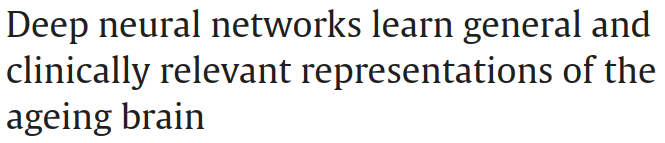
\includegraphics[width=8cm]{data/paper1.png}
                };
                \draw[red, thick] ($ (paper1.west) + (0.1, -0.25) $)-- ($ (paper1.west) + (3.5, -0.25) $);
                \node[text width=8cm, align=center, anchor=north, font=\tiny] at (paper1.south) {
                    \textit{Deep neural networks learn general and clinically relevant representations of the ageing brain}, Leonardsen et al., 2022. NeuroImage, 256, 119210
                };

                \node[draw=black, fill=white, inner sep=0pt] (paper3) at (0, -1.35) {
                    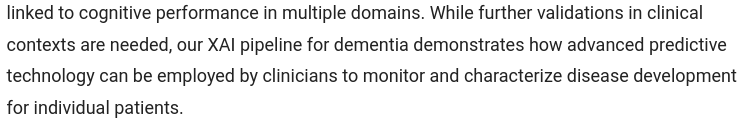
\includegraphics[width=8cm]{data/paper3.png}
                };
                \draw[red, thick] ($ (paper3.west) + (1.72, -0.28) $)-- ($ (paper3.west) + (3.63, -0.28) $);
                \node[fill=white, opacity=0.75, anchor=north west, minimum width=8cm, minimum height=0.3cm] at (paper3.north west) {};
                \node[text width=8cm, anchor=north] at (paper1.south) {};
                \node[fill=white, opacity=0.75, anchor=north west, minimum width=1.9cm, minimum height=0.3cm] at ($ (paper3.north west) - (0, 0.3) $) {};
                \node[text width=8.4cm, align=center, anchor=north, font=\tiny] at (paper3.south) {
                    \textit{Constructing personalized characterizations of structural brain aberrations}\\ \textit{in patients with dementia using explainable artificial intelligence},\\ Leonardsen et al., 2024.  npj Digital Medicine, 7(1), 110
                };
            }
            \visible<4-6>{
                \node[inner sep=0pt, draw=black, label=below:\tiny{https://github.com/estenhl/pyment-public}] (git) at (0, 0) {
                    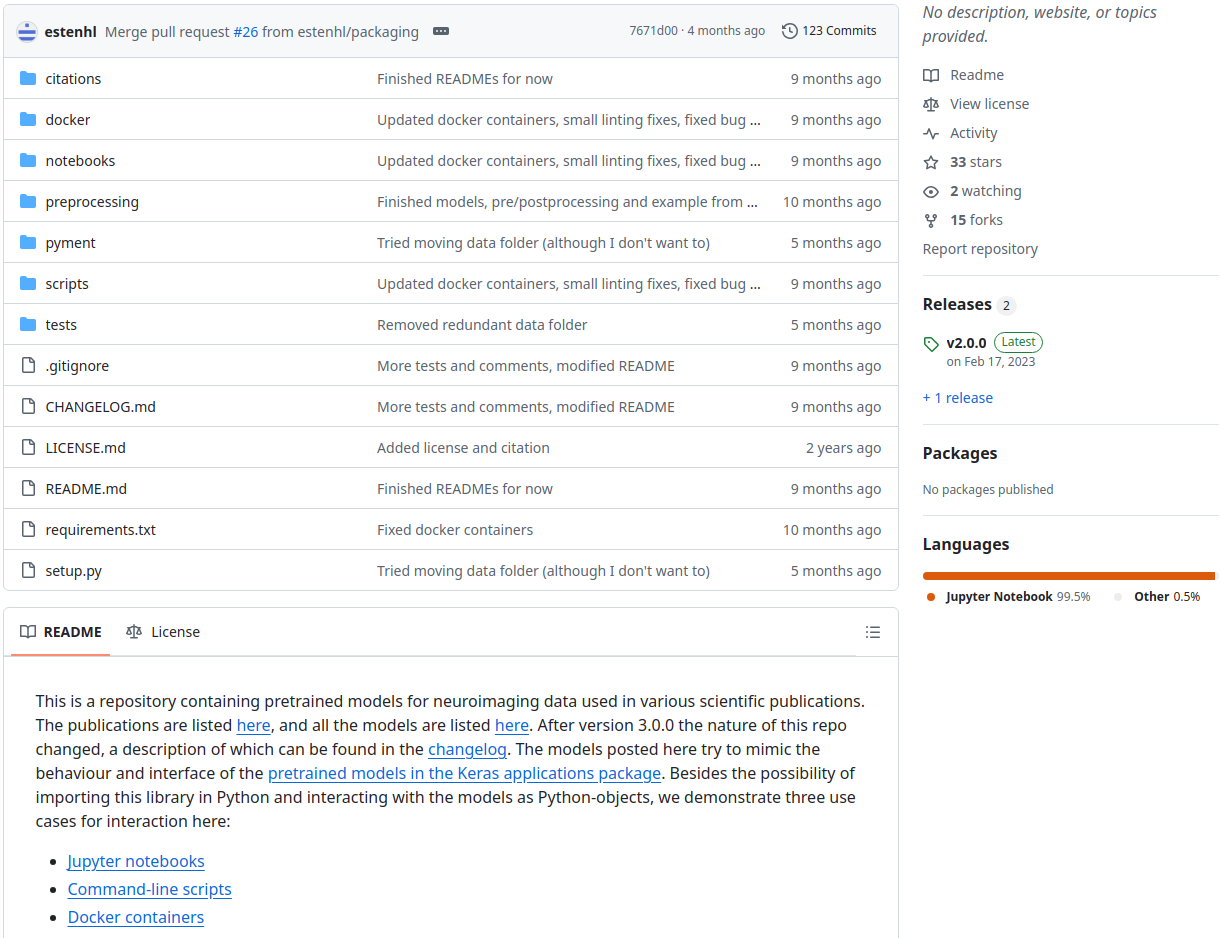
\includegraphics[width=9cm]{data/github.png}
                };
            }
            \visible<5>{
                \node[minimum width=0.7cm, minimum height=0.2cm, draw=red, very thick, inner sep=0pt] at ($ (git.east) - (1.9, -1.83) $) {};
            }
            \visible<6>{
                \node[minimum width=0.9cm, minimum height=0.2cm, draw=red, very thick, inner sep=0pt] at ($ (git.east) - (1.82, -2.69) $) {};
            }
            \visible<7-8>{
                \node[text width=10cm, font=\small] at (0, 0) {
                    \begin{enumerate}
                        \item Showcase the \textbf{general efficacy} of artificial intelligence for demonstrative clinical use-cases
                        \item<8> Build predictive models to solve specific \textbf{real-world clinical problems} using \textbf{commercially available data}
                        \item<8> Ensure the \textbf{robustness and utility} of the models through extensive validation
                        \item<8> Collaborate with clinicians to package the models in \textbf{user-friendly interfaces} integrating smoothly into \textbf{standardized clinical workflows}
                    \end{enumerate}
                };
            }
            \visible<9-10>{
                \node[] at (0, 0) {
                    Per
                };
            }
        \end{tikzpicture}
    \end{frame}

    \section{Decision support for neuroradiological examinations in dementia pre-diagnostics}

    \begin{frame}{Neuroradiological decision support}
        \centering
        \begin{tikzpicture}
            \visible<1>{
                \node[fill=white, draw=black] at (0, 0) {
                    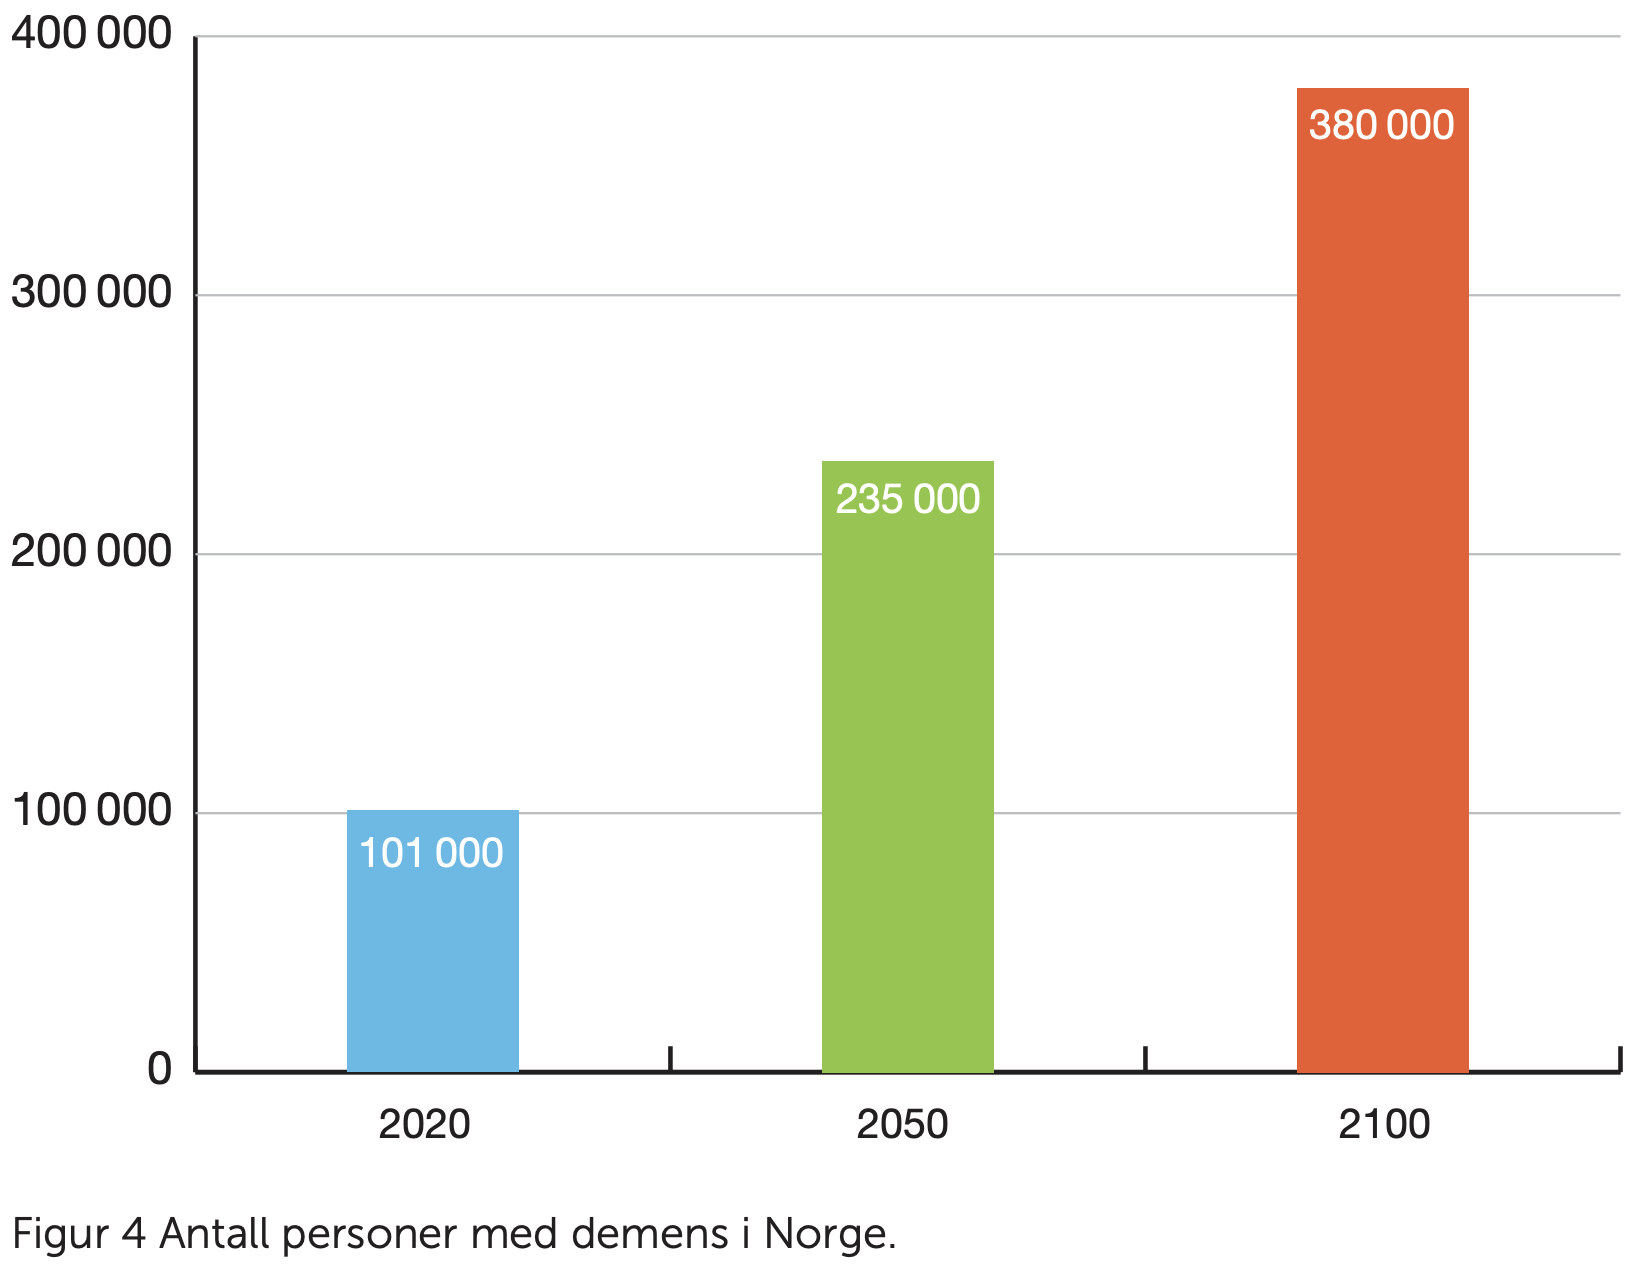
\includegraphics[width=8cm]{data/prevalence.png}
                };
            }
            \visible<2>{
                \node[] at (0, 0) {
                    Radiology time spent
                };
            }
            \visible<3>{
                \node[] at (0, 0) {
                    Subjectivity
                };
            }
            \visible<4>{
                \node[] at (0, 0) {
                    Tool demo
                };
            }
            \visible<5>{
                \node[] at (0, 0) {
                    Deep learning
                };
            }
            \visible<6>{
                \node[] at (0, 0) {
                    New treatments
                };
            }

        \end{tikzpicture}
    \end{frame}

    \section{Treatment response prediction and monitoring of patients on anti-amyloid therapies}

    \begin{frame}{Treatment response and monitoring}
        \centering
        \begin{tikzpicture}
            \visible<1>{
                \node[inner sep=0pt, draw=black] at (0, 0) {
                    
\includegraphics[width=9cm]{data/leqembi_ema.png}
                };
            }
            \visible<2>{
                \node[inner sep=0pt, draw=black] at (0, 0) {
                    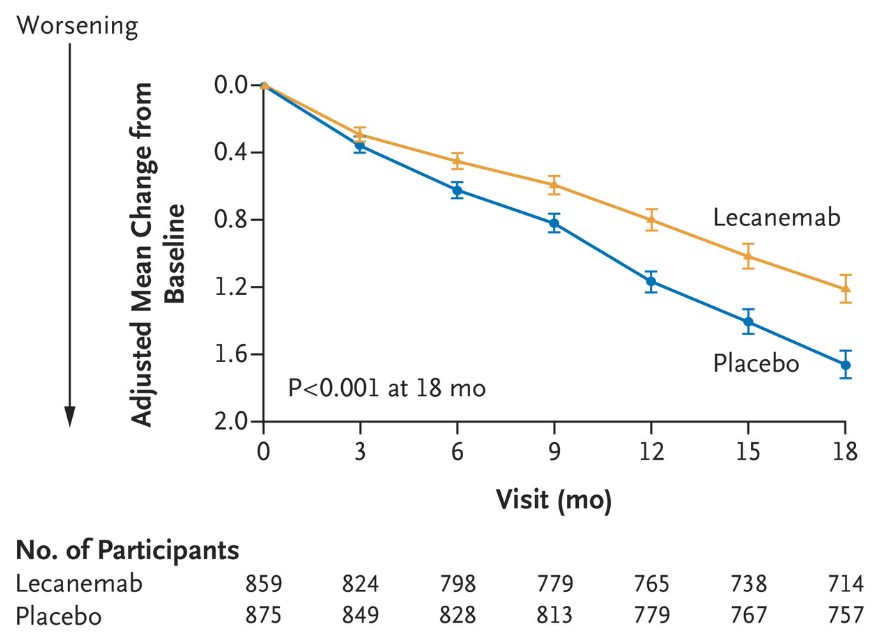
\includegraphics[width=7cm]{data/lecanemab.png}
                };
            }
        \end{tikzpicture}
    \end{frame}

\end{document}
